\begin{graphicspathcontext}{{./chapters/simulation/examples/imgs/},{./chapters/simulation/examples/imgs/auto/},\old}

\begin{frame}{Context}
	\smaller
	\begin{block}{Modeling and simulation of individuals in a large-scale virtual world}
	Reproduction of the dynamics of individuals and groups of individuals evolving in a large-scale virtual world (building, street\dots)
	\end{block}
	\vspace{2em}
	\begin{columns}
		\begin{column}[b]{.6\linewidth}
			\begin{block}{Application Domains}
			\begin{itemize}
			\item Development of urban sites, security study, flow analysis\dots
			\item Interactive staff training, serious games
			\item Video games, virtual animation\dots
			\end{itemize}
			\end{block}
		\end{column}
		\begin{column}[b]{.4\linewidth}
			\includegraphics{belfort_simulation}
		\end{column}
	\end{columns}
\end{frame}

\sidecite{Thalmann09}
\begin{frame}{Problems related to the simulation in virtual univers}
	\begin{enumerate}
	\item<1> Generating a population of virtual invividuals
	\vspace{1em}
	\item<1> Reproduction of the movements of the individuals
	\vspace{1em}
	\item<1> Generation of individual and collective behaviors
	\vspace{1em}
	\item<1,2> Modeling of a virtual environment
	\vspace{1em}
	\item<1> Interaction with the virtual population
	\vspace{1em}
	\item<1> Realistic displaying of the population and the univers
	\end{enumerate}
\end{frame}

\begin{frame}{Problematic}
	\smaller
	\begin{block}{Crowds and Traffic Simulation}
		\begin{itemize}
		\item enables the reproduction of the mobility behavior of individuals and groups of individuals
		\item may be applied on various types of environments (indoor/outdoor, open/closed space\dots)
		\end{itemize}
	\end{block}
	\begin{block}{Motivations}
		\begin{itemize}
		\item To provide accurate simulation for risk estimation and infrastructure design
		\item To enable to build communication media for stakeholders
		\end{itemize}
	\end{block}
	\begin{block}{Adopted Approach}
		\begin{itemize}
		\item Simulation of individuals $\Rightarrow$ Agent-based simulation.
		\end{itemize}
	\end{block}
\end{frame}

\begin{frame}{{Modeling and simulation} of virtual worlds}
	\smaller\smaller
	\begin{block}{Goals}
	Provide the tools for modeling and simulating entities of different types (vehicules, bicycles, pedestrians...) in a virtual world
	\end{block}
	\begin{block}{Constraints}
	\begin{description}
	\item Modeling and simulation relations \cite{Zeigler00}
	\item Minimize the simulator latency perceived by the immersed user (serious game)
	\item \alert{Minimize the design time of the environment model} that is built from geographical information systems and airplane photographies
	\end{description}
	\end{block}
	\begin{block}{Adopted approach}
	\begin{description}
	\item[Modeling] Adopt a graph-based model, which avoid redundancy in the model, and easy to edit
	\item[Simulation] Provide accurate and realtime implementation of the environment model, and of the individual behaviors
	\end{description}
	\end{block}
\end{frame}

\sidecite{Wilensky2015,Treuille2006,Shao2005,tecchia01platform}
\begin{frame}{Grid-based Modelling}
	\smaller
	\begin{block}{The environment is a grid}
		\begin{itemize}
		\item A cell contains a single object
		\item The agents are moving in 4 directions
		\item The agents may perceive on near cells
		\end{itemize}
	\end{block}
	\vspace{2em}
	\begin{columns}
		\begin{column}[t]{.7\linewidth}
			\inlineexamples{NetLogo, Jaak (Janus extension)\dots}
			\begin{alertblock}{But\dots}
				\begin{itemize}
				\item Discrete modeling of the environment: discrete perceptions and actions (motion, etc.)
				\item Limited size of the environment
				\item Not ``realistic''
				\end{itemize}
			\end{alertblock}
		\end{column}
		\begin{column}[t]{.3\linewidth}
			\raisebox{-\height}{\includegraphics{jaak_pacman}}
		\end{column}
	\end{columns}
\end{frame}

\begin{frame}[fragile]{Example of Grid Environment in SARL}
	\vspace{-1.5em}
	\begin{columns}
		\begin{column}[t]{.5\linewidth}
			\begin{sarllisting}[basicstyle=\tiny]
/* Object hierarchy */
class EnvObject {
  val id: UUID
  var x: int
  var y: int
}

class MobileObject
      extends EnvObject {
  var velocity: Vector2i
  var maxSpeed: float
}

class AgentBody
      extends MobileObject {
  var perception: Set<Perceivable>
  var influences: List<Influence>
  def applyInfluence(inf :
      Influence) {
    influences += inf
  }
}

/* Environment */
class Environment {
  val grid = <EnvObject>newArray
             (100,100)
  val bodies = <AgentBody>newHashSet
			\end{sarllisting}
		\end{column}
		\begin{column}[t]{.5\linewidth}
			\begin{sarllisting}[basicstyle=\tiny]
def computePerceptions {
  for (body : bodies) {
    body.perception = newSet
    for (i : -1 .. 1) {
      for (j : -1 .. 1) {
        var cell = grid.get(
            body.x + i, body.y + j)
        if (cell !== null) {
          body.perception += new
               Perceivable(cell)
        }}}}}

def updateEnvironment {
  for (body : bodies) {
    var resolvedInfluences = newSet
    for (inf : body.influences) {
      if (inf.inConflict(
          resolvedInfluences)) {
        inf = inf.resolve(
          resolvedInfluences)
      }
      resolvedInfluences += inf
    }
    for(reaction :
        resolvedInfluence) {
      reaction.apply(grid)
    }}}}
			\end{sarllisting}
		\end{column}
	\end{columns}
\end{frame}

\sidecite{Galland2011,Karamouzas2009,Doniec2008,Burghout04,Willemsen2003,Thomas2000}
\begin{frame}{Graph-based Modelling}
	\smaller
	\begin{block}{The environment is a graph}
		\begin{itemize}
		\item The road network is modeled with a graph
		\item The agents are moving along the graph (in 1D)
		\item The agents may perceive on near segments
		\end{itemize}
	\end{block}
	\vspace{2em}
	\begin{columns}
		\begin{column}[t]{.7\linewidth}
			\inlineexamples{S-Paramics, Aimsun, ArchiSim, Vissim, MatSim, Gama, JaSim (Janus extension)\dots}
			\begin{alertblock}{But\dots}
				\begin{itemize}
				\item Only for entities that follow paths (car, cycle, train\dots)
				\item Difficult to simulate motions in 2D
				\item Difficult to simulate vehicle overtaking
				\end{itemize}
			\end{alertblock}
		\end{column}
		\begin{column}[t]{.3\linewidth}
			\raisebox{-\height}{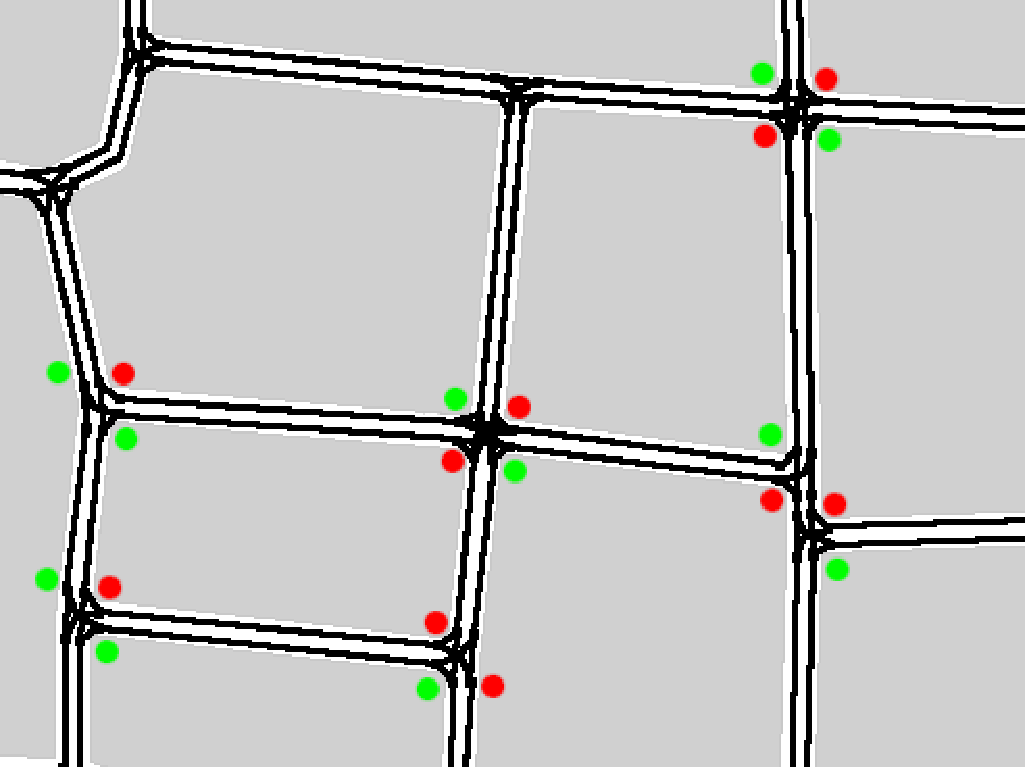
\includegraphics{3d-graph-example}}
		\end{column}
	\end{columns}
\end{frame}

\begin{frame}[fragile]{Example of Graph Environment in SARL}
	\vspace{-1cm}
	\begin{columns}
		\begin{column}[t]{.5\linewidth}
			\begin{sarllisting}[basicstyle=\tiny]
/* Graph */
class Edge {
  var start : Node
  var end : Node
  val objects : List<EnvObject>
}

class Node {
  val x : float
  val y : float
  var edges : List<Edge>
}

class Graph {
  val edges : List<Edge>
  val nodes : List<Node>
}

class EnvObject {
  val id : UUID
  var size : float
  var position : float
  var shiftingDistance : float
  var entry : Node
  var segment : Edge
}

/* Environment */
class Environment {
  val graph = new Graph
  val bodies = <AgentBody>newHashSet
			\end{sarllisting}
		\end{column}
		\begin{column}[t]{.5\linewidth}
			\begin{sarllisting}[basicstyle=\tiny]
def computePerceptions {
  for (body : bodies) {
    body.perception = newSet
    for (s : body.node.iterator(
      body.entry, position)) {
      for (o : s.objects) {
        body.perception += o
      }}}}

def updateEnvironment {
  for (body : bodies) {
  var resolvedInfluences = newSet
  for (inf : body.influences) {
    if (inf.inConflict(
        resolvedInfluences)) {
      inf = inf.resolve(
        resolvedInfluences)
    }
    resolvedInfluences += inf
  }
  for(reaction : resolvedInfluence){
    reaction.apply(grid)
  }}}}
			\end{sarllisting}
		\end{column}
	\end{columns}
\end{frame}

\sidecite{buisson.abmtrans13,Paris2007,Thalmann07,Braun05,Lamarche04}
\begin{frame}{Zone-based Modelling}
	\smaller
	\begin{block}{The environment is collection of inter-connected planar zones}
		\begin{itemize}
		\item Planar zones are built from the environment topology
		\item The agents are moving freely on a zone (in 2D)
		\item The agents perceive in the zones in intersection with their frustums
		\end{itemize}
	\end{block}
	\vspace{2em}
	\begin{columns}
		\begin{column}[t]{.7\linewidth}
			\inlineexamples{Place/Portal, PVS, Orca, ClearPath, JaSim (Janus extension)\dots}
			\begin{alertblock}{But\dots}
				\begin{itemize}
				\item Difficult to restrict motion
				\item Need complex algorithm to be built
				\item Need information related to the topology: road direction\dots
				\end{itemize}
			\end{alertblock}
		\end{column}
		\begin{column}[t]{.2\linewidth}
			\raisebox{-\height}{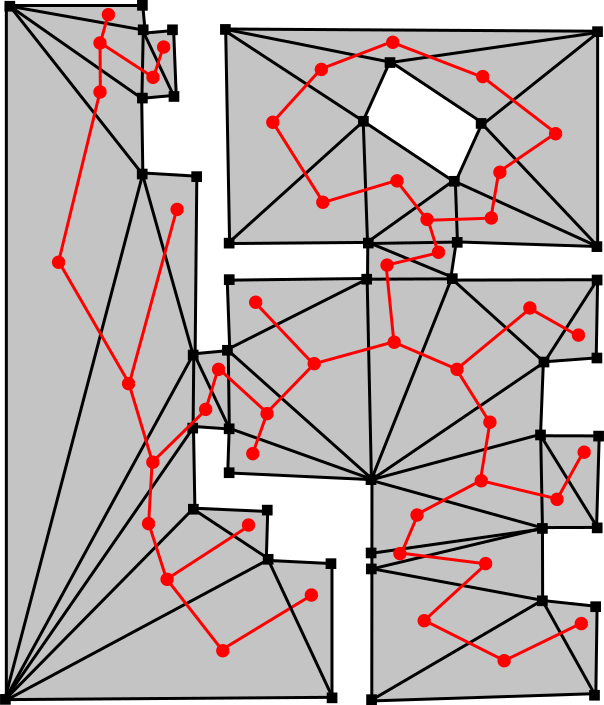
\includegraphics{3d-zones}}
		\end{column}
	\end{columns}
\end{frame}

\begin{frame}[fragile]{Example of Zone Environment in SARL}
	\vspace{-1cm}
	\begin{columns}
		\begin{column}[t]{.5\linewidth}
			\begin{sarllisting}[basicstyle=\tiny]
/* Zones */
class Zone {
  var shape : Shape2f
  var barycenter : Point2f
  var neightbors : Map<Segment2f,Zone>
  val objects : List<EnvObject>
}

class ZoneGraph {
  val zones : List<Zone>
}

class EnvObject {
  val id : UUID
  var box : Rectangle2f
  var position : Point2f
  var zone : Zone
}

/* Environment */
class Environment {
  val graph = new ZoneGraph
  val bodies = new HashSet<AgentBody>

  def computePerceptions {
    for (body : bodies) {
      body.perception = newSet
      for (z : body.zone.iterator(
               body.position)) {
        for (o : s.objects) {
			\end{sarllisting}
		\end{column}
		\begin{column}[t]{.5\linewidth}
			\begin{sarllisting}[basicstyle=\tiny]
          body.perception += o
        }
      }
    }
  }

  def updateEnvironment {
    for (body : bodies) {
      var resolvedInfluences = newSet
      for (inf : body.influences) {
        if (inf.inConflict(
            resolvedInfluences)) {
          inf = inf.resolve(
            resolvedInfluences)
        }
        resolvedInfluences += inf
      }
      for(reaction : resolvedInfluence){
        reaction.apply(grid)
      }
    }
  }
}
			\end{sarllisting}
		\end{column}
	\end{columns}
\end{frame}

\sidecite{GallandGaudDemangeKoukam2014_703,GallandGaudDemangeKoukam2009_11,Thalmann07,Farenc99}
\begin{frame}{Tree-based Modelling}
	\smaller
	\begin{block}{The environment is hierarchically decomposed into zones}
		\begin{itemize}
		\item Planar zones are built from a composition of a bigger zone
		\item The agents are moving freely on a zone (in 2D/3D)
		\item The agents perceive in the zones in intersection with their frustums
		\end{itemize}
	\end{block}
	\vspace{2em}
	\begin{columns}
		\begin{column}[t]{.7\linewidth}
			\inlineexamples{JaSim (Janus extension), Simulate\dots}
			\begin{alertblock}{But\dots}
				\begin{itemize}
				\item Tree data structure management is costly
				\item May be difficult to represent environment topology
				\item Need complex algorithm to be built
				\end{itemize}
			\end{alertblock}
		\end{column}
		\begin{column}[t]{.25\linewidth}
			\raisebox{-\height}{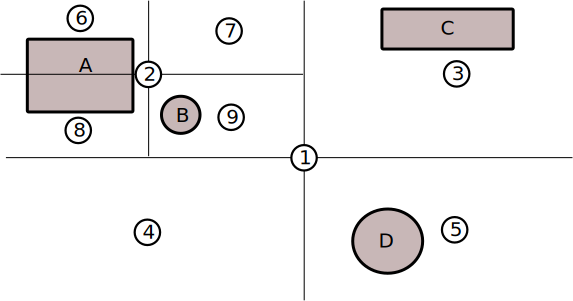
\includegraphics{tree_world}} \\[1em]
			\raisebox{-\height}{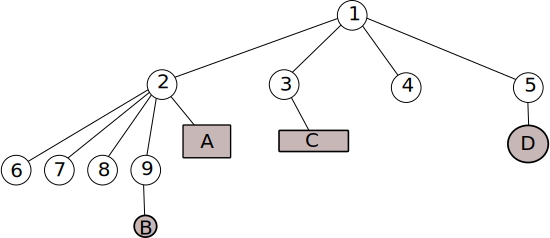
\includegraphics{tree_world_tree}} \\
		\end{column}
	\end{columns}
\end{frame}

\begin{frame}[t,fragile]{Example of Tree Environment in SARL}
	\vspace{-1.5em}
	\begin{columns}
		\begin{column}[t]{.5\linewidth}
			\begin{sarllisting}[basicstyle=\tiny]
/* Tree */
class TreeNode {
  var box : Rectangle2f
  var children : List<TreeNode>
  val objects : List<EnvObject>
}

class Tree {
  val root : TreeNode
  def iterator(frustum : Rectangle2f)
      : Iterator<EnvObject>
}

class EnvObject {
  val id : UUID
  var box : Rectangle2f
  var position : Point2f
  var node : TreeNode
}

/* Environment */
class Environment {
  val tree = new Tree
  val bodies = <AgentBody>newHashSet

  def computePerceptions {
    for (body : bodies) {
      body.perception = newSet
      for (o : tree.iterator(
           body.frustum)) {
			\end{sarllisting}
		\end{column}
		\begin{column}[t]{.5\linewidth}
			\begin{sarllisting}[basicstyle=\tiny]
        body.perception += o
      }
    }
  }

  def updateEnvironment {
    for (body : bodies) {
      var resolvedInfluences = newSet
      for (inf : body.influences) {
        if (inf.inConflict(
            resolvedInfluences)) {
          inf = inf.resolve(
	            resolvedInfluences)
        }
        resolvedInfluences += inf
      }
      for(reaction : resolvedInfluence){
        reaction.apply(grid)
      }
    }
  }
}
			\end{sarllisting}
		\end{column}
	\end{columns}
\end{frame}

\begin{frame}[fragile]{Iterators for Perception Computation (1/2)}
	\vspace{-1.5em}
	\begin{columns}
		\begin{column}[t]{.5\linewidth}
			\begin{sarllisting}[basicstyle=\tiny]
/*Iterator that replies the zones
  under intersection with the
  perception area */
class ZoneIterator
   implements Iterator<TreeNode> {

  val candidates = <TreeNode>
      newArrayList

  val frustum : Rectangle2f

  new (frustum : Rectangle2f,
       root : TreeNode) {
    this.frustum = frustum
    if (root.box.intersects(
        fustrum)) {
       candidates += root
    }
  }

  def hasNext : boolean {
    return ! candidates.empty
  }

  def next : TreeNode {
    var n = candidates.removeFirst
    for(c : n.children) {
      if (c.box.intersects(
          frustum)) {
			\end{sarllisting}
		\end{column}
		\begin{column}[t]{.5\linewidth}
			\begin{sarllisting}[basicstyle=\tiny]
        candidates += c
      }
    }
    return n
  }
}
/*Iterator that replies the
  objects under intersection
  with the perception area */
class PerceivableObjectIterator
   implements Iterator<EnvObject> {

  val candidates = <EnvObject>newArrayList

  val frustum : Rectangle2f
  val zones : Iterator<TreeNode>

  new (frustum : Rectangle2f,
       zones : Iterator<TreeNode>) {
    this.frustum = frustum
    this.zones = zones
    searchCandidates
  }

  def hasNext : boolean {
    return ! candidates.empty
  }
  /* ... */
			\end{sarllisting}
		\end{column}
	\end{columns}
\end{frame}

\begin{frame}[t,fragile]{Iterators for Perception Computation (2/2)}
	\vspace{-1.5em}
	\begin{columns}
		\begin{column}[t]{.5\linewidth}
			\begin{sarllisting}[basicstyle=\tiny]
  /* ... */

  def next : TreeNode {
    var n = candidates.removeFirst
    searchCandidates
    return n
  }

  def searchCandidates {
    while (candidates.empty
           && zones.hasNext) {

      var zone = zones.next

      for (o : zone.objects) {

        if (o.box.intersects(frustum)) {
		  candidates += o
		}

      }

    }

  }

}
			\end{sarllisting}
		\end{column}
		\begin{column}[t]{.5\linewidth}
			\mbox{}
		\end{column}
	\end{columns}
\end{frame}

\begin{frame}{Remaining Problems with Environment Models}
	\smaller
	\begin{block}{Problems}
		\begin{enumerate}
		\item Difficult for an entity to use different types of zones: \emph{how may a bicyclist follow a road, or traverse an open place with the same motion behavior?}
		\item Difficult to use the same zones for different types of entities: \emph{how to manage a bicyclist and a pedestrian on the same side-walk?}
		\item Difficult to manage perception and navigation, separatly.
		\item It is time consuming for designing.
		\end{enumerate}
	\end{block}
	\vspace{2em}
	\begin{alertblock}{Proposal \cite{Buisson2014b}}
		\begin{itemize}
		\item Definition of the environment model based on the an hybrid zonal/graph representation.
		\item Provide tools for easy edition (based on the SIMULATE\textup{\regmark} framework).
		\end{itemize}
	\end{alertblock}
\end{frame}

\end{graphicspathcontext}
